\documentclass[10pt, a4paper, twocolumn]{article}
\input{structure.tex}
\addbibresource{references.bib}
\title{Implementing Sensorless Field Oriented Control: A Case Study}

\author{
	\authorstyle{Shin Umeda}
}


\date{\today} 

\begin{document}

\maketitle 

\thispagestyle{firstpage} 

\lettrineabstract{Lorem ipsum dolor sit amet, consectetur adipiscing elit, sed do eiusmod tempor incididunt ut labore et dolore magna aliqua. Ut enim ad minim veniam, quis nostrud exercitation ullamco laboris nisi ut aliquip ex ea commodo consequat. Duis aute irure dolor in reprehenderit in voluptate velit esse cillum dolore eu fugiat nulla pariatur. Excepteur sint occaecat cupidatat non proident, sunt in culpa qui officia deserunt mollit anim id est laborum.}

\section{Background}
The principle goal of the SJSU Robotics club is to build robots. In order to improve supply-chain resiliance and reduce dependence on vendors, the SJSU Robotics Electrical Engineering Sub-team has created a motor controller (hereon "Perseus") that is agnostic to the motor itself.

The primary issues faced when using servo motors were: \begin{enumerate}
  \item Inability to debug firmware
  \item Inability to reflash or update firmware
  \item Lack of diagnostics
  \item Difficulty with physical repair
  \item Difficulty with support due to differing timezones
  \item Difficulty with sourcing due to geopolitical shifts
\end{enumerate}

Many of these issues were not inherent to any motor or vendor in particular, and would not be improved by changing vendor. Motor firmware is usually highly proprietary, and thus most vendors do not provide a means to debug the firmware. Furthermore, the historically the team has sourced motors from China. Due to recent geopolitical shifts, this has become rather infeasible.

Furthermore, our own BLDC driver board would provide many advantages. We would be able to write our own firmware, and be able to choose how we interface with it as we wish. We can also offload additional tasks onto the motor, such as detecting limit-switch activations. We can also freely choose whatever motor we wish, adapting the motor the the mechanical requirements.

For these reasons, along with academic curiosity, we have chosen to create our own motor driver. Our motor driver uses modern algorithms to achieve fully sensorless Field Oriented Control, allowing for maximum mechanical flexibility.

\section{Theory of Operation}
BLDC theory
\subsection{Brushless DC Motors}

\begin{figure}
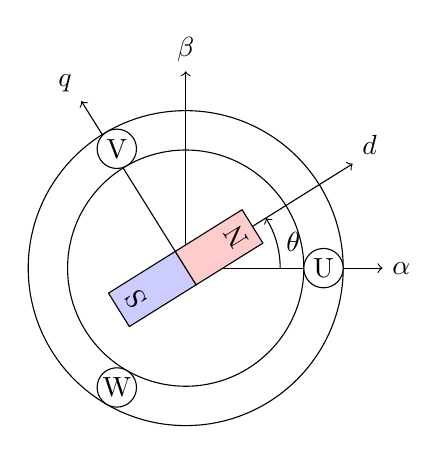
\begin{tikzpicture}
\draw[->](0, 0) -- (0:2.5) node[right]{$\alpha$};
\draw[->](0, 0) -- (90:2.5) node[above]{$\beta$};
\draw[->](0, 0) -- (32:2.5) node[above right]{$d$};
\draw[->](0, 0) -- (122:2.5) node[above left]{$q$};
\draw (0,0) circle [radius=2];
\draw (0,0) circle [radius=1.5];
\draw[fill=white] (0:1.75) circle [radius=0.25] node{U};
\draw[fill=white] (120:1.75) circle [radius=0.25] node{V};
\draw[fill=white] (240:1.75) circle [radius=0.25] node{W};
\filldraw[fill=blue!20,rotate=32] (-1, -0.25) rectangle (0, 0.25);
\filldraw[fill=red!20,rotate=32] (0, -0.25) rectangle (1, 0.25);
\node[rotate=122] (N) at (32:0.75){N};
\node[rotate=122] (S) at (32:-0.75){S};
\draw[->](1.2,0) arc (0:32:1.2) node[midway, right] {$\theta$};
\end{tikzpicture}
\caption{A simplified single pole-pair three-slot BLDC motor with coordinate systems labeled.}
\label{motor}
\end{figure}

Brushless DC Motors can be described as having two parts: a stationary stator
and a rotating rotor. The stator possesses electromagnet coils which move the
magnets stuck on the rotor. As seen in figure \ref{motor}, the stator coils have
three phases: u, w, v. The coils are wired together in a wye configuration, meaning
that the sum of the currents of the phases is zero (barring leakage or shorts).

\begin{equation}
\vec{\tau}=\vec{m}\times\vec{B}=\vert m\vert\vert B\vert sin(\theta)
\label{motor_torque}
\end{equation}

Brushless DC Motors are different in comparison to Brushed DC motors, in that
their commutation is done electronically.  As is well known, the torque of a motor is the cross product of the magnetic dipole moment and the magnetic field. (Eq. \ref{motor_torque}) This means to maximize torque, the magnetic field must be oriented $90^\circ$ to the rotor. Much of the difficulty in doing so is determing the rotor position and calculating the math for the necessary current in real time.

\subsection{Clarke-Park Transform}

The Clarke transform, otherwise known as the $\alpha\beta\gamma$ transform, converts three-phase current (referred to hereon out as the $uvw$ space) to $\alpha\beta\gamma$ space. $\alpha\beta\gamma$ space is significantly more convenient because it transforms three sine waves offset by $60^\circ$ to two sine waves offset by $90^\circ$ degrees.

\begin{equation}
\begin{bmatrix}
  i_{\alpha} \\
  i_{\beta} \\
  i_{\gamma}
\end{bmatrix}
  =T\vec{i}_{uvw}=\sqrt{\frac{2}{3}}\begin{bmatrix}
    1 & -\frac{1}{2} & -\frac{1}{2} \\
    0 & \frac{\sqrt{3}}{2} & -\frac{\sqrt{3}}{2} \\
    \frac{1}{\sqrt{2}} & \frac{1}{\sqrt{2}} & \frac{1}{\sqrt{2}}
  \end{bmatrix}
  \begin{bmatrix}
    i_{u} \\
    i_{v} \\
    i_{w}
  \end{bmatrix}
  \label{clarke}
\end{equation}

As seen in Eq. \ref{clarke}, the first and second rows are made up of the
three-phase vector's contributions to the x and y axis. The third row is
the sum of all of the currents, and is zero unless the currents are unbalanced.

\begin{equation}
  T\begin{bmatrix}
    i\sin(\theta) \\
    i\sin(\theta + \frac{2}{3}\pi) \\
    i\sin(\theta + \frac{4}{3}\pi)
  \end{bmatrix}=\begin{bmatrix}
     i\sin(\theta) \\
     i\cos(\theta) \\
     0
  \end{bmatrix}
\end{equation}

Notably, in a balanced system the $\gamma$ term can be ignored since we assume current cannot leak out of the system. In order to use this for rotor control however, we need to maintain a flux $90^\circ$ from the rotor. In other words, the current vector must be perpendicular to the rotor. In order to seperate the perpendicular and the on-axis components, we rotate the coordinate system by the angle of the rotor. This is the Park trasform. (Eq. \ref{park})

\begin{equation}
  i_{dq0}=
  \begin{bmatrix}
    \cos(\theta) & -\sin(\theta) \\
    \sin(\theta) & \cos(\theta)
  \end{bmatrix}
  \begin{bmatrix}
    i_{\alpha} \\
    i_{\beta}
  \end{bmatrix}
  \label{park}
\end{equation}

The Park transform transforms a $\alpha\beta$ vector into a $dq0$ vector. A $dq0$ vector has two components: the direct component, and the quadrature component. The direct component is current in-axis with the rotor, while the quadrature component is perpendicular to the rotor and actually provides torque. To maximize efficiency then, we must minimize the direct component while controlling the quadrature component for torque.

\subsection{Field Oriented Control}

The field oriented control algorithm is as such: we first determine our rotor angle through some means. We then measure the current of the phases of the motor. We transform the current using the Clarke-Park transform to find a direct and quadrature current. We use a PID controller to minimize direct current, and to set quadrature current to some desired torque value. The resulting output values are then inverse Clarke-Park transformed into sine values, which are then fed into an H-bridge to control the motor. (Fig. \ref{FOC-control})

\newcommand{\mixer}[2]{
    \draw circle[radius=#1, #2] (45:-#1) -- (45:#1) (135:-#1) -- (135:#1)
}

\begin{figure}
  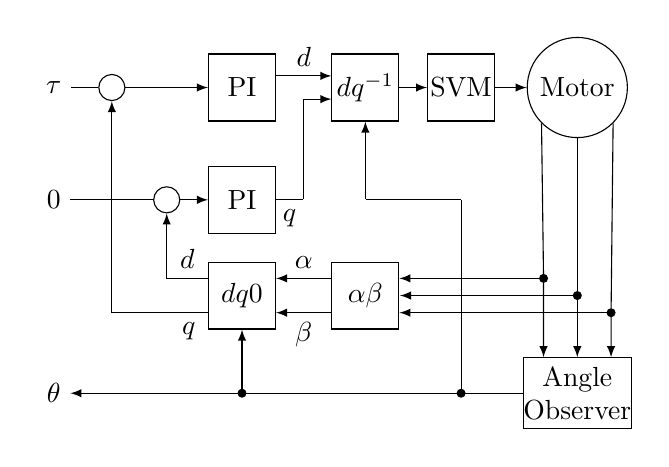
\begin{tikzpicture}[node distance=5mm,
                    rect/.style={draw, rectangle,minimum size=8.5mm, inner xsep=0mm, align=center, node distance = 1},
                    circ/.style={draw, circle,minimum size=2mm, align=center, node distance = 2},
                    arrow/.style={draw, -latex,node distance=2cm},
                    sum/.style={draw, circle, node distance = 1},
                    coord/.style={minimum size = 0,inner sep=0},
                    tap/.style={minimum size = 1, inner sep = 1, draw, circle, fill=black},]
  \matrix[row sep=10,column sep=10]{
  \node(torque){$\tau$}; &
  \node(sum_q)[sum]{}; &&
  \node(q_pid)[rect]{PI} node at (q_pid.east)(q_pid_e)[coord, inner ysep=4]{}; &
  \node(p00)[coord, inner ysep = 4]{}; &
  \node(inv_dq)[rect]{$dq^{-1}$} node at (inv_dq.west)(inv_dq_w)[coord, inner ysep=4]{}; &
  \node(svm)[rect]{SVM}; &
  \node(motor)[circ]{Motor}; \\
  \node(dref){0}; &&
  \node(sum_d)[sum]{}; &
  \node(d_pid)[rect]{PI}; &
  \node(p10)[coord]{}; &
  \node(p11)[coord]{}; &
  \node(p12)[coord]{}; \\
  &\node(p0)[coord, inner ysep = 6]{};
  &\node(p1)[coord, inner ysep = 6]{};
  & \node(dq)[rect]{$dq0$} node at (dq.west) (dq_w)[coord, inner ysep = 6]{} node at (dq.east) (dq_e)[coord, inner ysep=6]{};
  &&\node(ab)[rect]{$\alpha\beta$} node at (ab.west)(ab_w)[coord, inner ysep=6]{} node at (ab.east)(ab_e)[coord, inner ysep=6]{}; &&
  \node(taps)[coord, inner ysep=6, inner xsep=12]{} node at (taps.north west)(ta)[tap]{} node at (taps)(tb)[tap]{} node at (taps.south east)(tc)[tap]{}; \\
  \node(ang){$\theta$}; &&&
  \node(p33)[tap]{}; &&&
  \node(p35)[tap]{}; &
  \node(obv)[rect]{Angle\\Observer} node at (obv.north)(obv_n)[coord, inner xsep=12]{}; \\
  };
  \draw[arrow] (obv) -> (ang);
  \draw[arrow] (motor.south west)  -- (ta) -- (obv_n.west);
  \draw[arrow] (motor) -- (tb) -- (obv);
  \draw[arrow] (motor.south east) -- (tc) -- (obv_n.east);
  \draw[arrow] (torque) -> (sum_q) -> (q_pid);
  \draw[arrow] (q_pid_e.north) -> (inv_dq_w.north) node[above, midway]{$d$};
  \draw[arrow] (d_pid.east) -- (p10) node[below, midway]{$q$} -- (p00.south) --(inv_dq_w.south);
  \draw[arrow] (inv_dq)->(svm);
  \draw[arrow] (svm)->(motor);
  \draw[arrow] (ta) -- (ab_e.north);
  \draw[arrow] (tb) -- (ab_e);
  \draw[arrow] (tc) -- (ab_e.south);
  \draw[arrow] (dq_w.north) -- (p1.north) node[above, pos=0.5]{$d$} -- (sum_d);
  \draw[arrow] (dq_w.south) -- (p0.south) node[below, pos=0.2]{$q$} -- (sum_q);
  \draw[arrow] (ab_w.north) -- (dq_e.north) node[above, midway]{$\alpha$};
  \draw[arrow] (ab_w.south) -- (dq_e.south) node[below, midway]{$\beta$};
  \draw[arrow] (dref) -- (sum_d) -- (d_pid);
  \draw[arrow] (p33) -- (dq.south);
  \draw[arrow] (p35) -- (p12) -- (p11) -- (inv_dq.south);
  \end{tikzpicture}
  \caption{FOC Control Loop}
  \label{FOC-control}
\end{figure}

\subsubsection{Space Vector Modulation}

Notably however, the inverse Clarke-Park transform is not the best way to control the motor. The maximum magnitude output by such a transform is $\sin(60^\circ)$ of the input voltage, which is about 86\% of the input voltage. This discrepancy comes from the fact that at no point are all of the switchs' PWM at 100\%. i.e. when at $\theta=0$, phase u would be at 100\%, but phases w and v would be at -86\%. Space Vector Control gets around this by not outputing sine waves, but instead breaking down the space into 6 vectors and switching between vectors. Depending on angle, it chooses two vectors as the components and switches between the two. This makes it possible to PWM one vector at 100\%, maintaining 100\% duty cycle and making full use of our voltage range. TODO insert graphic.

\subsection{Sensorless Rotor Measurement}

Notably, Field Oriented Control requires constant measurement of the rotor position. This requires either a quadrature encoder, which introduces a mechanical point of failure and additional mounting hardware, or a magnetic encoder, which is typically bottlenecked by the communication protocol and/or has too slow of a sample rate to be useful.While not insurmountable, these issues require additional care concerning the motor used. In order to be truly motor-agnostic, it is then necessary to consider sensorless motor sensing.

The architecture we have chosen to use combines a sensorless flux linkage algorithm with a high frequency injection algorithm to provide position detection for low and high speeds. The flux linkage algorithm uses motor characteristic knowledge to derive back EMF from current, which is then used to estimate rotor position. When rotor speeds are too slow to provide significant back EMF, high frequency injection is used.

\subsubsection{Flux Linkage Observer}

The Flux Linkage observer is the MXLEMMINGS observer from the \cite{MESC_MAN}, with a few additions from \cite{simplefoc2022}. As is well known, the voltage of a motor
is proportional to the change of magnetic flux over time. In other words, the
magnetic flux of a motor is the integral of the voltage of the motor over time. (Eq. \ref{fluxemf})

\begin{equation}
  \vec{\psi}=\int \vec{V}_{\text{BEMF}} dt + \vec{C}
  \label{fluxemf}
\end{equation}

Fortunately, we can determine motor back EMF voltage from current alone using knowledge of the motor characteristics. (TODO insert circuittikz motor model). As is well known, a motor can be electrically modeled as three components: the resistivity of the coils, the inherent inductance of the coils, and a voltage source from the back EMF. It then follows, that the voltage of a motor can be described like in equation \ref{motoreq}.

\begin{equation}
  V_m=Ri+L\frac{di}{dt}-V_{\text{BEMF}}
  \label{motoreq}
\end{equation}

Since we already know the voltage of the motor (as we are applying said voltage), we need only measure current and change in current to determine back EMF. The flux linkage observer does as such and retrieves the angle of the resulting flux vector to determine rotor angle.

The flux linkage observer however, comes with two major infirmities: an inability to determine initial rotor position, and a dependence on back EMF. When back EMF is very small, such as when the rotor speed is slow, the flux linkage observer fails to determine back EMF from noise. Furthermore, the flux linkage observer can only integrate a change in angle, and is unable to determine initial angle. To suppliment these weaknesses, high frequency injection is used in conjunction with flux linkage observance.

\subsubsection{High Frequency Injection}

The firmware describes high frequency injection as described by \cite{SUN20226457}. High frequency injection depends on a critical characteristic of the rotor referred to as saliency. Saliency can be described by how the rotor inductance changes depending on angle. By injecting high frequency pulses of current, and measuring the resulting impedance, we can deduce the inductance of the rotor at that angle. Then we use saliency to determine angle from the inductance.

First, we begin by transforming everything into the $dq0$ coordinate system. High frequency injection detects the error between estimated angle and the real angle, and to do so we need to rotate everything by the estimated angle so we can find error. Once we have our rotating reference frame, we first inject voltage into the system.
\begin{equation}
  \begin{bmatrix}
    v_{d} \\
    v_{q}
  \end{bmatrix}=
  \begin{bmatrix}
    Z_d & 0 \\
    0 & Z_q
  \end{bmatrix}
  \begin{bmatrix}
    i_d \\
    i_q
  \end{bmatrix}
  \label{dq_impedance}
\end{equation}

That said, we do not have the real rotor position, so we cannot find $\hat{i}$ or $\hat{v}$ in $dq0$ space. By rotating the estimated vectors, we can get the real vectors.

\begin{equation}
  \hat{v} =
  \begin{bmatrix}
    \cos(\Delta\theta) & -\sin(\Delta\theta) \\
    \sin(\Delta\theta) & \cos(\Delta\theta)
  \end{bmatrix}v
  \label{rot_v}
\end{equation}
\begin{equation}
  \hat{i} =
  \begin{bmatrix}
    \cos(\Delta\theta) & -\sin(\Delta\theta) \\
    \sin(\Delta\theta) & \cos(\Delta\theta)
  \end{bmatrix}i
  \label{rot_i}
\end{equation}

By substituting equations \ref{rot_v} and \ref{rot_i} and inverting the impedance matrix, it follows that we end up with equation \ref{dq_err}, where $Z=(Z_d + Z_q) / 2$ and $\Delta Z=(Z_d - Z_q) / 2$.

\begin{equation}
 \hat{i}=
  \frac{1}{Z_d Z_q}
  \begin{bmatrix}
    Z - \Delta Z\cos(2\Delta\theta) & -\Delta Z\sin(2\Delta\theta) \\
    -\Delta Z\sin(2\Delta\theta) & Z + \Delta Z\cos(2\Delta\theta)
  \end{bmatrix}
  \hat{v} 
  \label{dq_err}
\end{equation}

To minimize disturbing the torque of the motor, we always inject volage into the d axis and never inject any into the q axis. As such we can set $\hat{v}_q$ to 0. Furthermore, we are trying to minimize error, so we choose to measure only $\hat{i}_q$ since it becomes zero when $\Delta\theta=0$ and $\hat{v}_q=0$. We inject $\hat{v}_q=V_h\cos(\omega_h t)$, where $\omega_h$ is the frequency of the high frequency injection and $V_h$ is the magnitude. From this, we find $\hat{i}_q$ in terms of $\Delta\theta$ and $\hat{v}_q$ in equation \ref{iq_wave}.

\begin{equation}
  \hat{i}_q
 = \frac{-\Delta Z V_h\cos(\omega_h t)}{Z_d Z_q}\sin(2\Delta\theta) 
 \label{iq_wave}
\end{equation}

Notably however, this is a sine wave, and therefore useless as an error signal. In order to extract the signal ($\sin(2\Delta\theta$), we need to extract it from the sine wave. We demodulate the signal via superheterodyning as demonstrated in \cite{dmytrohfi}, shown in figure (TODO insert tikz plot of heterodyning). This error signal is input into a phase locked loop consisting of a PI controller and an integrator. (TODO insert another tikz plot) This phase locked loop will converge on the correct angle.

TODO need to check if initial rotor position detection is necessary as described in \cite{SUN20226457}. \cite{dmytrohfi} makes no reference of it, and seemingly implies that it will always convege on the true angle. Given \cite{SUN20226457} uses a simplified saliency model which leaves an ambiguity whereas \cite{dmytrohfi} does not, it would imply for motors with more than one pole pair it should be fine. Further testing required.

\section{Implementation}

Perseus is a small motor control board consisting of a DRV8300 three-phase H-bridge, hall effect current sensors, integrated CAN bus, and a micromod microcontroller slot. The DRV8300 H-bridge driver was chosen due to its simplicity, which allows for flexibility. For example, earlier prototypes of Perseus was used as a brushed motor driver, which would have been impossible if the H-bridge driver handled commutation. The usage of a simplistic H-bridge driver also allows us to implement commutation in software.

The usage of a micromod slot is due to the SJSU robotics club's ecosystem, and allows for swapping the microcontroller on the fly. This means an in-circuit programmer is not necessary, and microcontrollers can be swapped out for performance or repair. The CAN bus is the standard interface used on our robots, and uses the SN65 3.3V CAN transciever. CANbus is expected to be implemented in hardware on the microcontroller, or in software.

\section{Firmware}

The FOC library is a low level toolkit for controlling BLDC motors. It provides both open loop and closed loop FOC control as well as multiple angle observers. It utilizes hardware PWM timers instead of software PWM to reduce the computation demands of FOC. A typical use case consists of a fast FOC loop, a slower position/velocity PID loop, and a slower event handling loop.

The FOC loop needs to be the fastest since it must respond to the rotation of the rotor, which can easily exceed hundreds of radians per second. Current measurements and angle estimation is fed into the FOC control algorithm, which adjusts PWM duty cycles using either SVM or sine wave output. The mechanical control loop is significantly slower, as position/velocity is expected to be slower than the rotor due to gear ratios. Then an event loop handles high level control signals, such as setpoint changes or PID tuning.

\printbibliography[title={Bibliography}] 



\end{document}
